\section{Resultados ilustrativos}
\label{sec:resultados}

Todos os números desta secção são \textbf{gerados automaticamente} por \texttt{npm run paper:figures} a partir do motor \texttt{runSimulation} do repositório. As figuras usam \texttt{pgfplots} lendo ficheiros CSV exportados pelo mesmo script, de modo que pequenos ajustes de parâmetros podem refletir-se rapidamente no PDF.

% Gerado por scripts/generate-paper-figures.ts
\newcommand{\StatCompletedA}{7}
\newcommand{\StatMeanCtA}{2.71}
\newcommand{\StatMedianCtA}{3.00}
\newcommand{\StatCompletedB}{7}
\newcommand{\StatMeanCtB}{2.57}
\newcommand{\StatMedianCtB}{2.00}
\newcommand{\StatCompletedC}{7}
\newcommand{\StatMeanCtC}{3.00}
\newcommand{\StatMedianCtC}{3.00}
\newcommand{\StatCompletedD}{7}
\newcommand{\StatMeanCtD}{2.71}
\newcommand{\StatMedianCtD}{3.00}


A Figura~\ref{fig:cfdA} mostra a dinâmica de filas no cenário A: como o estoque em \texttt{backlog} se relaciona com o trabalho em progresso nas colunas de especialidade. As Figuras~\ref{fig:bar} e~\ref{fig:tp} resumem comparações entre cenários: a primeira destaca o tempo de ciclo médio (a mediana complementa a Tabela~\ref{tab:resumoCenarios}), enquanto a segunda mostra diferenças de \emph{throughput} por sprint quando o padrão de sinergia entre pares muda.

\begin{figure}[htbp]
  \centering
  % Generated by scripts/generate-paper-figures.ts
\begin{tikzpicture}
\begin{axis}[
  width=0.95\linewidth,
  height=5.4cm,
  xmin=1,
  xlabel={Dia global},
  ylabel={Cartões por coluna},
  legend columns=3,
  legend style={font=\scriptsize,at={(0.5,1.02)},anchor=south},
]
\addplot[thick,const plot,color=black!70] table[col sep=comma,x=day,y=backlog]{data/cfd_A_baseline.csv};
\addplot[thick,const plot,color=violet!80] table[col sep=comma,x=day,y=analise]{data/cfd_A_baseline.csv};
\addplot[thick,const plot,color=teal!80] table[col sep=comma,x=day,y=dev]{data/cfd_A_baseline.csv};
\addplot[thick,const plot,color=orange!90] table[col sep=comma,x=day,y=teste]{data/cfd_A_baseline.csv};
\addplot[thick,const plot,color=red!80] table[col sep=comma,x=day,y=deploy]{data/cfd_A_baseline.csv};
\legend{Backlog,Análise,Dev,Testes,Deploy}
\end{axis}
\end{tikzpicture}

  \caption{Contagens de cartões por coluna ao longo dos dias globais no cenário A (referência).}
  \label{fig:cfdA}
\end{figure}

\begin{figure}[htbp]
  \centering
  % Generated by scripts/generate-paper-figures.ts
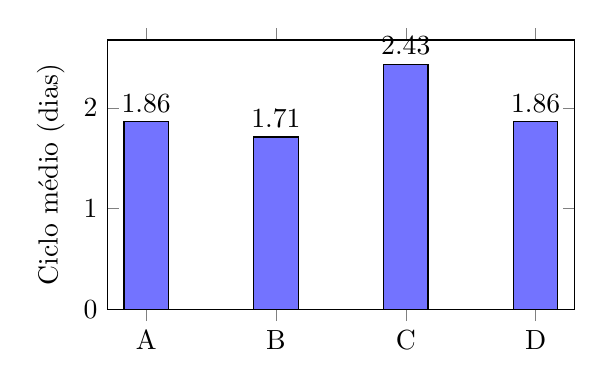
\begin{tikzpicture}
\begin{axis}[
  width=0.62\linewidth,
  height=5cm,
  ybar,
  ymin=0,
  symbolic x coords={A,B,C,D},
  xtick=data,
  xticklabel style={align=center},
  ylabel={Ciclo médio (dias)},
  nodes near coords,
  nodes near coords align={vertical},
  bar width=16pt,
]
\addplot[fill=blue!55] coordinates {(A,1.86) (B,1.71) (C,2.43) (D,1.86)};
\end{axis}
\end{tikzpicture}

  \caption{Tempo de ciclo médio (dias) por cenário, considerando apenas cartões concluídos na janela simulada.}
  \label{fig:bar}
\end{figure}

\begin{figure}[htbp]
  \centering
  % Generated by scripts/generate-paper-figures.ts
\begin{tikzpicture}
\begin{axis}[
  width=0.95\linewidth,
  height=5.2cm,
  xlabel={Sprint},
  ylabel={Cartões concluídos},
  xmin=1,
  xmax=10,
  ymin=0,
  legend style={font=\scriptsize,at={(0.5,1.02)},anchor=south},
  legend columns=4,
]
\addplot[thick,mark=*,color=black!70] table[col sep=comma,x=sprint,y=A]{data/throughput_by_sprint.csv};
\addplot[thick,mark=square*,color=blue!70] table[col sep=comma,x=sprint,y=B]{data/throughput_by_sprint.csv};
\addplot[thick,mark=triangle*,color=red!75] table[col sep=comma,x=sprint,y=C]{data/throughput_by_sprint.csv};
\addplot[thick,mark=diamond*,color=teal!80] table[col sep=comma,x=sprint,y=D]{data/throughput_by_sprint.csv};
\legend{A,B,C,D}
\end{axis}
\end{tikzpicture}

  \caption{\emph{Throughput} por sprint (cartões que chegam a \texttt{deploy} nessa sprint) para os quatro cenários.}
  \label{fig:tp}
\end{figure}

\begin{table}[htbp]
  \centering
  \caption{Resumo dos quatro cenários (ciclo médio e mediano em dias; valores gerados em \texttt{summary\_stats.tex}).}
  \label{tab:resumoCenarios}
  \begin{tabular}{@{}lccc@{}}
    \toprule
    Cenário & Concluídos & Ciclo médio & Ciclo mediano \\
    \midrule
    A & \StatCompletedA & \StatMeanCtA & \StatMedianCtA \\
    B & \StatCompletedB & \StatMeanCtB & \StatMedianCtB \\
    C & \StatCompletedC & \StatMeanCtC & \StatMedianCtC \\
    D & \StatCompletedD & \StatMeanCtD & \StatMedianCtD \\
    \bottomrule
  \end{tabular}
\end{table}

\paragraph{Leitura rápida.}
No pacote aqui reportado, o cenário B tende a melhorar o tempo de ciclo médio em relação a A quando a colaboração em \texttt{dev} é amplificada, enquanto o cenário C piora a média ao combinar um \emph{repasse} desfavorável com maior propensão a retrabalho. O cenário D combina os dois efeitos de $S$ e permite discutir interação entre canais de sinergia para a mesma semente e \emph{backlog}.

Ficheiros adicionais em \texttt{paper/figures/} (SVG) e \texttt{paper/data/} (CSV/JSON) permitem reproduzir gráficos fora do \LaTeX{}.
